\chapterformat{Results}
In this chapter, we present the results of predicting the eigenfrequency response of the membrane to a given mass distribution using the developed simulation framework.

\section{Basic Results}
\label{sec:basic_results}

We first show basic simulation results, including the displacement field obtained from the elasticity PDE, as well as the modeshapes and eigenfrequencies obtained from the wave PDE. 
Example runs can be generated using \texttt{demo.ipynb}.\\

The simulation begins by solving the elasticity PDE for the displacement field $\fatu$. From this, the stress field is computed as $\fatsig = \fatsig_u + \fatsig_p$, which serves as the input to the wave PDE. Both fields are shown in Figure \ref{fig:disp_and_stress} for the default parameter set. 
Comparing the stress field to the prestress distribution in Figure \ref{fig:density_and_prestress} reveals that the elasticity equation redistributes the increased prestress on the electrodes across a larger area, thereby reducing the stress directly on the electrodes. While the corners of the membrane exhibit strong peaks, these remain numerically stable.  

\begin{figure}[h]
    \centering
    \begin{overpic}[height=\domainheight]{figures/pngs/displacement.png}
        \put(12,60){\large\bfseries\textcolor{white}{A}}
    \end{overpic}%
    \hfill
    \begin{overpic}[height=\domainheight]{figures/pngs/stress_field.png}
        \put(12,60){\large\bfseries\textcolor{white}{B}}
    \end{overpic}
    \caption{(\textbf{A}) Norm of the displacement field $\fatu$. (\textbf{B}) Norm of the resulting stress field $\fatsig$.}
    \label{fig:disp_and_stress}
\end{figure}

Using the stress field $\fatsig$ shown in Figure \ref{fig:disp_and_stress}, we next solve the wave PDE. Our primary interest lies in the eigenfrequencies of the membrane, since these can be directly compared to the experimentally measured resonant frequencies. Such a comparison provides a meaningful assessment of the accuracy of the model. 
For this purpose, we use experimental data obtained from a physical membrane, as discussed in detail in section \ref{sec:measurements}.  
The prestress $\sigma_\silnit$ was determined by fitting the $(1,1)$ mode frequency, yielding $\sigma_\silnit=\SI{27.8}{\mega\pascal}$. A comparison of simulated eigenfrequencies with the measured data is shown in Figure \ref{fig:std_params}.  

\begin{figure}[h]
    \centering
    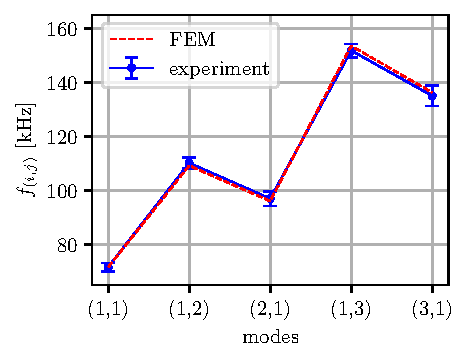
\includegraphics[]{figures/parameter_analysis/para_ana_standard.pdf}
    \caption{Eigenfrequencies obtained with default parameters compared to experimental data. The prestress of the simulation was fitted to $\sigma_\silnit=\SI{27.8}{\mega\pascal}$.}
    \label{fig:std_params}
\end{figure}

The simulated eigenfrequencies agree with the experimental data within the respective error bounds, supporting the validity of the model.\\

Finally, Figure \ref{fig:modeshapes} illustrates selected eigenmodes obtained from the wave PDE. The modeshapes demonstrate how the electrodes break the ideal symmetry of the membrane. Figuratively, the peaks of the modeshapes are “attracted” toward the additional mass of the electrodes. This is particularly visible in the $(3,1)$ mode, where the peaks near the electrodes are noticeably shifted inward. In section \ref{sec:other_modeshapes}, we will observe a similar “attraction” effect caused by deposited sample mass.

\newpage

\begin{figure}[h]
    \centering
    \begin{tabular}{cc}
        % Row 1
        \begin{overpic}[height=\domainheight]{figures/pngs/modeshape_(1,1).png}
        \put(9,86){\large\bfseries\textcolor{white}{(1,1)}}
    \end{overpic}&
        \begin{overpic}[height=\domainheight]{figures/pngs/modeshape_(2,2).png}
        \put(9,86){\large\bfseries\textcolor{white}{(2,2)}}
    \end{overpic}\\
        % Row 2
        \begin{overpic}[height=\domainheight]{figures/pngs/modeshape_(2,1).png}
        \put(9,86){\large\bfseries\textcolor{white}{(2,1)}}
    \end{overpic}&
        \begin{overpic}[height=\domainheight]{figures/pngs/modeshape_(1,2).png}
        \put(9,86){\large\bfseries\textcolor{white}{(1,2)}}
    \end{overpic}\\
        % Row 3
        \begin{overpic}[height=\domainheight]{figures/pngs/modeshape_(3,1).png}
        \put(9,86){\large\bfseries\textcolor{white}{(3,1)}}
    \end{overpic}&
        \begin{overpic}[height=\domainheight]{figures/pngs/modeshape_(1,3).png}
        \put(9,86){\large\bfseries\textcolor{white}{(1,3)}}
    \end{overpic}\\
    \end{tabular}
    \caption{Selected modeshapes of the membrane with default parameters. The color scale is omitted, since the absolute vibration amplitudes depend on the excitation energy and are not fixed in the eigenvalue problem.}
    \label{fig:modeshapes}
\end{figure}

\newpage

\subsection{Other Modeshapes}
\label{sec:other_modeshapes}

The simulation parameters strongly influence the resulting modeshapes. Two representative cases are shown in Figure \ref{fig:other_modeshapes}.  
Compared to Figure \ref{fig:modeshapes}, the $(1,3)$ mode with altered electrode parameters and higher prestress (fitted for membranes from another manufacturer, see section \ref{sec:other_prestress}) exhibits a split of the upper and lower peaks. This degeneracy prevents correct identification by our mode detection algorithm and would require a more specialized approach.  
In the $(3,1)$ mode with deposited sample mass, the central peak is visibly shifted toward the coffee-ring deposit. Although the peak is close to splitting, the detection algorithm still succeeds in this case. With larger mass or a wider coffee ring radius, however, the peak would likely split further, causing the algorithm to fail.  

\begin{figure}[h]
    \centering
    \begin{tabular}{cc}
        % Row 1
        \begin{overpic}[height=\domainheight]{figures/pngs/modeshape_(1,3)_degenerate.png}
        \put(9,86){\large\bfseries\textcolor{white}{(1,3) degenerate}}
    \end{overpic}&
        \begin{overpic}[height=\domainheight]{figures/pngs/modeshape_(3,1)_sampled.png}
        \put(9,86){\large\bfseries\textcolor{white}{(3,1) with sample}}
    \end{overpic}\\
    \end{tabular}
    \caption{Modeshapes under modified conditions. Left: $(1,3)$ mode with altered electrode parameters ($\sigma_\silnit=\SI{84.9}{\mega\pascal}$, $h_\gold=\SI{85}{\nano\meter}$, $h_\chro=\SI{5}{\nano\meter}$). Right: $(3,1)$ mode with a sampled mass of $40\ ng$ in coffee ring (default parameters, $\sigma_\silnit=\SI{27.8}{\mega\pascal}$). The mesh is shown to indicate the position of the deposited mass.}
    \label{fig:other_modeshapes}
\end{figure}


\newpage
\section{Parameter Analysis}
\label{sec:parameter_analysis}

Appendix \ref{sec:remarks_parameter_analysis} gives some remarks on this section.\\

In this section we analyze the effect of individual simulation parameters on the eigenfrequencies. For each parameter, we compare the default setting with both a decreased and an increased value. The results are shown in Figure \ref{fig:para_ana}. The parameter variations were chosen such that their effects are clearly visible in the plots, allowing us to build intuition for their influence. For comparison, we use unsampled membranes produced by the same manufacturer (Invisible Light Labs) as the sampled membranes.\\
Throughout this section, the membrane prestress is fixed at $\sigma_\silnit=\SI{27.8}{\mega\pascal}$, the value determined in section \ref{sec:basic_results}.\\
The corresponding results can be reproduced with \texttt{parameter\_analysis.ipynb} and \texttt{parameter\_search.ipynb}. The default parameter set yields the results in Figure \ref{fig:std_params}. Two main deviations from an ideal homogeneous membrane can be observed:\\
First, the $(1,2)$ and $(2,1)$ modes differ in frequency, as do their higher-order analogues. Since the perforation is symmetric with respect to both axes, this asymmetry must be entirely due to the electrodes.\\
Second, the spacing between successive modes is not uniform. Specifically, the frequency increase from $(1,1)$ to $(2,1)$ is smaller than that from $(2,1)$ to $(3,1)$. A similar effect is visible for the $(1,2)$ and $(1,3)$ modes. This indicates that the perforation affects the first and third modes more strongly than the second ones. In the default parameter set, the perforation only reduces the effective mass, which raises the eigenfrequencies (as opposed to non-default parameters where a change in perforation prestress is imposed).\\

\subsection{Membrane thickness}
Figure \ref{fig:para_ana} (A) shows the effect of varying the membrane thickness.\\
Changing the thickness alters the relative significance of membrane mass and prestress compared to the electrode mass and prestress.\\
The $(2,1)$ and $(3,1)$ modes are most strongly affected, consistent with their stronger interaction with the electrodes. By contrast, the $(1,1)$, $(1,2)$, and $(1,3)$ modes remain essentially unchanged. This is expected, since in the case of an ideal membrane the eigenfrequencies are independent of thickness (see section \ref{sec:assumptions}).\\

\subsection{Radius of the perforation}
Figure \ref{fig:para_ana} (B) shows the influence of the perforation radius.\\
When the radius changes, the electrode geometry changes as well, since the percentage of free area $P_\mathrm{el}$ is fixed and thus the electrode area increases as the perforation radius decreases.\\
Increasing the perforation radius increases the eigenfrequencies, as the total effective mass decreases.\\
A striking feature is the behavior of the $(3,1)$ frequency, which is affected in the opposite direction. A possible explanation is that enlarging the perforation radius shifts the electrodes closer to the membrane boundary, aligning them with the side peaks of the $(3,1)$ mode. This increases the effective mass of the $(3,1)$ mode and thereby reduces its frequency.\\

\subsection{Mass percentage of the perforation}
Figure \ref{fig:para_ana} (C) shows the effect of varying the perforation mass percentage.\\
An increased perforation mass percentage increases the effective system mass, thus lowering the eigenfrequencies.\\
The relative effect is slightly larger for the $(1,1)$, $(1,2)$, and $(1,3)$ modes than for the $(2,1)$ and $(3,1)$ modes. The latter are also influenced by the electrodes, whose effect is not altered by the perforation mass. Surprisingly, the frequency shifts are very similar across all modes, with only minor differences.\\
The effect is somewhat stronger for the first and third modes, likely because the peaks of the second modes overlap less with the perforation.\\

\subsection{Prestress on the perforation}
Figure \ref{fig:para_ana} (D) shows the effect of varying the effective prestress on the perforation.\\
Our physical intuition suggests that the effective prestress on the perforation should equal that of the unperforated membrane. Nevertheless, we test the effect explicitly.\\
As expected, increasing the effective prestress raises the eigenfrequencies.\\
Unexpectedly, the $(1,1)$ mode shows virtually no dependence on the perforation prestress.\\

\subsection{Thickness of $\gold$}
Figure \ref{fig:para_ana} (E) shows the effect of varying the $\gold$ layer thickness.\\
Since the bulk of the electrode mass is in the $\gold$ layer, changing its thickness primarily affects electrode mass.\\
Increasing electrode mass lowers the eigenfrequencies. Interestingly, the $(1,2)$ and $(1,3)$ modes are also significantly influenced, despite limited overlap with the electrodes.\\
The electrode mass affects the $(2,1)$ and $(3,1)$ modes more strongly than the $(1,2)$ and $(1,3)$ modes, consistent with greater overlap. The relative change is larger for $(2,1)$ than for $(3,1)$, which is somewhat surprising since the electrodes coincide more directly with the $(3,1)$ side peaks. A possible explanation is that the central peak of the $(3,1)$ mode does not overlap with the electrodes, reducing the net effect.\\

\subsection{Thickness of $\chro$}
Figure \ref{fig:para_ana} (F) shows the effect of varying the $\chro$ layer thickness.\\
Since the electrode prestress is governed mainly by the $\chro$ layer, changing its thickness alters the electrode prestress.\\
Increasing the electrode prestress raises the eigenfrequencies.\\
Unexpectedly, the effect is weaker for the $(2,1)$ and $(3,1)$ modes than for the others, even though the electrodes act more directly on them. A possible explanation is that while electrode mass primarily affects the $(2,1)$ and $(3,1)$ modes (due to overlap with peaks), the electrode prestress acts more strongly on the $(1,2)$ and $(1,3)$ modes due to the electrodes behaving like a prestressed string aligned along the $y$-direction, thereby supporting those modes.\\

\newpage

\begin{figure}[h]
    \centering
    \setlength{\tabcolsep}{2pt}
    \begin{tabular}{cc}
        % Row 1
        \begin{overpic}[]{figures/parameter_analysis/para_ana_hsin.pdf}
        \put(15,69){\large\bfseries\textcolor{black}{A}}
    \end{overpic}&
        \begin{overpic}[]{figures/parameter_analysis/para_ana_Rperf.pdf}
        \put(9,74){\large\bfseries\textcolor{black}{B}}
    \end{overpic}\\
        % Row 2
        \begin{overpic}[]{figures/parameter_analysis/para_ana_mpercentage_perf.pdf}
        \put(15,69){\large\bfseries\textcolor{black}{C}}
    \end{overpic}&
        \begin{overpic}[]{figures/parameter_analysis/para_ana_sigpercentage_perf.pdf}
        \put(9,74){\large\bfseries\textcolor{black}{D}}
    \end{overpic}\\
        % Row 3
        \begin{overpic}[]{figures/parameter_analysis/para_ana_hau.pdf}
        \put(15,75){\large\bfseries\textcolor{black}{E}}
    \end{overpic}&
        \begin{overpic}[]{figures/parameter_analysis/para_ana_hcr.pdf}
        \put(9,81){\large\bfseries\textcolor{black}{F}}
    \end{overpic}\\
    \end{tabular}
    \caption{Eigenfrequencies of the simulation under parameter variations. Experimental results are shown translucently as the solid blue curve.}
    \label{fig:para_ana}
\end{figure}


\newpage



\subsection{Parameter search}
\label{sec:parameter_search}
The aim of this section is to explore which sets of parameters yield the best agreement between simulation and experiment. Two groups of parameters are not well constrained a priori: (i) the effective parameters of the perforation and (ii) the electrode layer thicknesses. For the perforation parameters, it is not clear whether the assumptions made are entirely accurate, while for the electrode layers, the nominal values from the manufacturer cannot be verified precisely by measurement. Thus, both sets of parameters are optimized here.\\

We define a loss function $L:\mathbb{R}^2 \rightarrow \mathbb{R}$ that quantifies the deviation between experiment and simulation for two varied parameters $P_1$ and $P_2$:
\[
L(P_1,P_2)=\sum\limits_{\{e\}} \sum\limits_{\{ m\}} \big| f_{e,m} - f_{\mathrm{FEM},e,m}(P_1,P_2) \big|,
\]
where $f_{e,m}$ is the measured frequency of mode $m$ for experiment $e$, and $f_{\mathrm{FEM},e,m}(P_1,P_2)$ the corresponding simulated frequency with parameters $(P_1,P_2)$. The set $\{e\}$ contains experiments on membranes from three different manufacturers, ensuring that the optimization does not simply “overfit” to one particular sample. The set $\{ m\}$ contains the five lowest modes: $\{(1,1),(2,1),(1,2),(3,1),(1,3)\}$.\\

In some cases, not all modes could be detected experimentally, and thus the loss could not be computed for these modes. This introduces a slight bias, but does not affect the overall conclusions. As discussed in section \ref{sec:other_modeshapes}, mode detection may fail in cases where the eigenmodes become degenerate or distorted.\\

For each experiment, the $\silnit$ prestress was set such that $f_{\mathrm{FEM},e,(1,1)}=f_{e,(1,1)}$. Later in this section, we further discuss why this is a methodologically sound approach. The evaluation of $L$ is computationally expensive, as it requires running a simulation for each experiment and each parameter configuration. Nevertheless, we conducted a grid search to explore the parameter dependence in detail.\\

The loss with default parameters is
\[
L_\mathrm{std}=\SI{19.1 \pm 39.1}{\kilo\hertz}.
\]
Again, within the error bounds of the experiments this is essentially zero, so the parameter search is not strictly necessary.\\

\subsubsection{Effective perforation parameters}
\label{sec:para_search_eff_perf}

We varied the effective perforation parameters $\{\sigma_{\mathrm{eff}}^*,\rho_{\mathrm{eff}}^*\}$ in a small domain around their default values. The results are shown in figure \ref{fig:loss_landscapes} (B).\\

On the given grid, we found the minimum:
\begin{align*}
    L(\sigma_\mathrm{eff}^*=0.95, \rho_\mathrm{eff}^*=0.70)&=\SI{11.1\pm39.1}{\kilo\hertz}\\
\end{align*}

Interestingly, the loss landscape forms a valley extending from high to low values of $\sigma_\mathrm{eff}^*$ and from low to high values of $\rho_\mathrm{eff}^*$. This indicates that an increase in effective density can be compensated by a decrease in effective prestress. At first sight, this appears counterintuitive, since both effects would normally be expected to reduce the eigenfrequencies. The explanation lies in the fact that a third parameter, the membrane prestress $\sigma_\silnit$, is not fixed but determined by fitting the $(1,1)$ mode to the experimental data. Consequently, a decrease in $\sigma_\mathrm{eff}^*$ leads to an increased fitted value of $\sigma_\silnit$, which in turn raises the eigenfrequencies. While this procedure may seem methodologically questionable—since the physical prestress of the membrane is not actually changing—the true value of $\sigma_\silnit$ is unknown a priori. Thus, the value obtained from fitting with the default parameters is not necessarily closer to the physical prestress than the one obtained when adapting the effective parameters. It is entirely plausible, for example, that the effective prestress of the perforation is $\sigma_\mathrm{eff}^*=0.9$, in which case the true membrane prestress would be larger than the value inferred from the default parameters. Nevertheless, since the default parameters lie close to the observed minimum and, when experimental uncertainties are taken into account, are equivalent to it, we retain the default parameter set.\\


The observation that the best agreement is obtained for values of $\sigma_\mathrm{eff}^*$ close to $1$ provides strong support for the initial assumption regarding this parameter. Prior to the parameter search, it was not evident whether an alternative choice, such as $\sigma_\mathrm{eff}^*=0.62$ by analogy with $\rho_\mathrm{eff}^*$, might also be justified. The results clearly indicate that this is not the case.\\


\subsubsection{Electrode thicknesses}

We next varied the electrode thicknesses $h_\chro$ and $h_\gold$ around their default values. The resulting loss landscape is shown in Figure \ref{fig:loss_landscapes} (A). A valley can be observed parallel to the $h_\chro$ axis, indicating that the $\chro$ thickness has only a minor effect on the results. In contrast, the gold layer thickness has a more significant impact.\\

The minimum loss on the given grid was found at
\begin{align*}
    L(h_\gold=\SI{90}{\nano\meter}, h_\chro=\SI{8.7}{\nano\meter})&=\SI{16.5\pm39.1}{\kilo\hertz}\\
\end{align*}
which is only slightly smaller than the default loss. Since the effect is minor and the minimum lies close to the default parameters, we retain the default electrode thicknesses in subsequent simulations.\\

\begin{figure}[h]
    \centering
    \begin{tabular}{cc}
        \begin{overpic}[]{figures/loss_landscape_el_thickness.pdf}
        \put(33,88){\large\bfseries\textcolor{white}{A}}
        \end{overpic}&
        \begin{overpic}[]{figures/loss_landscape_eff_perf.pdf}
        \put(27,65){\large\bfseries\textcolor{white}{B}}
        \end{overpic}\\
    \end{tabular}
    \caption{Loss landscapes. (\textbf{A}) Electrode thickness. Simulations did not converge for some parameter sets; these points are left blank. (\textbf{B}) Effective perforation parameters. The color scale is capped at \SI{50}{\kilo\hertz}, although some values exceed this range.}
    \label{fig:loss_landscapes}
\end{figure}






\section{Membranes with Other Parameters}
\label{sec:other_parameters}

In addition to the default membranes, devices with different production parameters were available. Specifically, we investigated membranes with higher prestresses and membranes of different lateral dimensions than the default size of $1\ \mathrm{mm}$. In this section, we compare the corresponding experimental measurements with the FEM results in order to validate the simulation across a broader parameter space. The results can be reproduced using \texttt{other\_parameters.ipynb}.\\

\subsection{Prestress}
\label{sec:other_prestress}
So far, the reference values were taken from membranes fabricated by Invisible-Light Labs. To further validate the model, we compared the FEM simulations with membranes from other manufacturers exhibiting substantially different prestress values. As shown in Figure \ref{fig:other_prestress}, the agreement between experiment and simulation remains within the error bounds. The only notable deviation is the $(2,1)$ mode in Figure \ref{fig:other_prestress} (A), which can be attributed to the exceptionally small experimental uncertainty.\\


\begin{figure}[h]
    \centering
    \begin{tabular}{cc}
        % Row 1
        \begin{overpic}[]{figures/other_parameters_Norcada.pdf}
        \put(15,75){\large\bfseries\textcolor{black}{A}}
    \end{overpic}&
        \begin{overpic}[]{figures/other_parameters_MS.pdf}
        \put(10,80){\large\bfseries\textcolor{black}{B}}
    \end{overpic}\\
    \end{tabular}
    \caption{Comparison of experimental and simulated eigenfrequencies for membranes from different manufacturers with different prestresses. (\textbf{A}) Higher prestress, manufacturer Norcada \cite{Norcada}. (\textbf{B}) Slightly higher prestress, manufacturer MS.}
    \label{fig:other_prestress}
\end{figure}

\subsection{Membrane Size}
\label{sec:membrane_size}
In addition to the standard $1\ \mathrm{mm}$ membranes, devices with side lengths of $0.5\ \mathrm{mm}$ were also measured. Figure \ref{fig:sizes} shows the comparison of the FEM simulations with the experimental data for the $0.5\ \mathrm{mm}$ membranes. The simulations reproduce the measured eigenfrequencies of the first and second modes well, confirming the robustness of the model. Unfortunately, the third modes could not be measured on these membranes.\\


\begin{figure}[h]
    \centering
    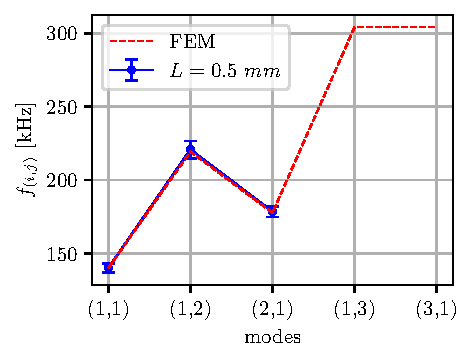
\includegraphics[]{figures/other_parameters_half_size.pdf}
    \caption{FEM results compared to experimental data for membranes with a side length of $0.5\ \mathrm{mm}$. The simulation was performed with a prestress of $\sigma_\silnit = \SI{28.0}{\mega\pascal}$. The $(3,1)$ mode has not been correctly labelled by the mode detection algorithm.}
    \label{fig:sizes}
\end{figure}





\section{Measurements}
\label{sec:measurements}

In the scope of this thesis, we measured the eigenfrequencies of EMILIE membranes with and without deposited materials. In this section, we present the results of these measurements. Note that these are not the only measurements performed: additional unsampled membranes were used in sections \ref{sec:parameter_analysis} and \ref{sec:other_parameters} for calibration and validation of the FEM model.  

The eigenfrequency measurements were carried out using a Polytec MSA-500. For each deposited chemical and mass, three membranes from the same production batch were characterized. We report the mean eigenfrequency of each triplet, with the error bars given by the standard deviation. The sampled membranes were taken from the same batch as used in \cite{timaracpopovic25}. Since that study focused on IR absorption, the eigenfrequencies without IR excitation were not recorded, and we therefore performed them here. Unfortunately, no unsampled membranes from this batch were retained. Earlier measurements exist, but their eigenfrequencies are systematically higher, likely due to relaxation effects over time. This is not a major limitation, since the eigenfrequency shifts induced by small deposited masses are negligible; we therefore assume that the unsampled membranes would exhibit frequencies close to those of the membranes carrying the smallest mass of $625\ \mathrm{pg}$.


We note that the assignment of measured peaks to eigenmodes involves some degree of uncertainty. Each measurement was performed by sweeping a frequency range of interest and recording the membrane response spectrum with the Polytec PSV software. In some cases, the correspondence between spectral peaks and eigenmodes was ambiguous, so occasional misassignments cannot be excluded.  

The eigenfrequencies of membranes sampled with polystyrene (PS) and polypropylene (PP) are shown in Figure \ref{fig:mass_response}. For PS, the eigenfrequency response exceeds the estimated simulation uncertainty (see section \ref{sec:parameter_analysis}) only for deposited masses above \SI{10}{\nano\gram}, while for PP no significant effect is observed at any mass. This constitutes one of the key results of this thesis: a purely mechanical FEM simulation does not approximate the system with sufficient accuracy to capture the effect of deposited masses below \SI{10}{\nano\gram}. Since the EMILIE device targets this regime, the approach developed here is not directly applicable in practice. In the following chapters we will nevertheless examine, in a quantitative manner, the predictive capability of the simulation.  

\begin{figure}[h]
    \centering
    \begin{overpic}[]{figures/exp_freqs_sampled_PS.pdf}
        \put(10,47){\large\bfseries\textcolor{black}{A}}
    \end{overpic}\\[0.5em]
    \begin{overpic}[]{figures/exp_freqs_sampled_PP.pdf}
        \put(10,51){\large\bfseries\textcolor{black}{B}}
    \end{overpic}
    \caption{Measured eigenfrequencies of sampled membranes. 
    (\textbf{A}) Membranes with deposited Polystyrene (PS). A clear downshift of the eigenfrequencies is observed only for deposited masses of \SI{10}{\nano\gram} and above; below this threshold, the frequency shifts remain within the measurement error. 
    (\textbf{B}) Membranes with deposited Polypropylene (PP). Within the studied mass range, no systematic shift of the eigenfrequencies is detectable, indicating that the influence of PP deposition is below the sensitivity limit of the measurement. 
    In both cases, the results highlight that the current simulation approach cannot reliably resolve mass loadings in the sub-\SI{10}{\nano\gram} range.}

    \label{fig:mass_response}
\end{figure}






\section{Simulation results for added masses}

We now compare the simulation results for membranes with added masses to the corresponding experimental data. Since the experimental observations differ fundamentally between PS and PP, they are discussed separately. For PS, the data suggests that the deposited material carries little to no prestress. In contrast, the PP data indicates that the deposited material induces a significant prestress, which we attempt to model in the following.\\
As discussed in section \ref{sec:measurements}, no data is available for unsampled membranes of the corresponding batch. We therefore determined the membrane prestress using a chip with the smallest PP sample mass. The chip with \SI{625}{\pico\gram} PP yielded a prestress of \SI{27.1}{\mega\pascal}, which we then used as the reference value for all further simulations, including those with PS.\\

\subsection{Polystyrene}
\label{sec:polystyrene}

The results in this section were generated with \texttt{sample\_mass\_analysis.ipynb}. Simulation data was collected for added masses between \SI{625}{\pico\gram} and \SI{40}{\nano\gram}, matching the available experimental values. The coffee-ring deposits formed from the droplets varied somewhat in radius and shape, but microscopy revealed that they were approximately circular with a radius of about \SI{200}{\micro\meter}, centered on the perforation. The primary variation was in the ring width, which we implemented in the simulations according to table \ref{tab:coffee_ring_widths}, derived from microscope images.\\

\begin{table}[h]
    \centering
    \begin{tabular}{|c|c|c|c|c|c|c|c|}
        \hline
        Mass [pg] & 625 & 1250 & 2500 & 5000 & 10000 & 20000 & 40000 \\
        \hline
        Ring width [$\mu m$] & 10 & 10 & 12 & 12 & 15 & 16 & 22 \\
        \hline
    \end{tabular}
    \caption{Ring widths of PS coffee-ring deposits, extracted from microscopy images.}
    \label{tab:coffee_ring_widths}
\end{table}

As a first comparison, Figure \ref{fig:mass_response_fem} (A) shows the simulation results overlayed with the experimental PS data, assuming zero prestress in the deposited material. The agreement is reasonable overall. The main discrepancy occurs for the $(3,1)$ mode, which may stem either from a measurement error (e.g. misassignment of a spectral peak) or from physical effects not captured by the present model. Figure \ref{fig:mass_response_fem} (B) provides a clear visual comparison between the simulation results and the experimental data. The simulation does not lie entirely within the standard deviation of the measurements, which would represent the ideal agreement; however, the deviation remains relatively small.
\\


\begin{figure}[h]
    \centering
    \begin{overpic}[]{figures/fem_freqs_sampled_PS.pdf}
        \put(10,50){\large\bfseries\textcolor{black}{A}}
    \end{overpic}\\
    \hspace*{-.5cm}%
    \begin{overpic}[]{figures/mean_abs_fem_exp_difference_sampled.pdf}
        \put(9,55){\large\bfseries\textcolor{black}{B}}
    \end{overpic}
    \caption{(\textbf{A}) Raw data of simulated eigenfrequencies of membranes with PS deposits compared to experimental data (shown translucently). The simulations assume zero prestress in the deposited material. (\textbf{B}) Relative difference of the simulated eigenfrequencies to the experimental eigenfrequencies. The standard deviation of the experimental data is shown in gray.}
    \label{fig:mass_response_fem}
\end{figure}

To better visualize the trends, we analyze the relative frequency shifts. For each mode (except $(3,1)$), we calculate the relative shift $f_r=(f_s-f_u)/f_u$, where $f_s$ and $f_u$ denote the sampled and unsampled eigenfrequencies, respectively. Error bars are determined by Gaussian error propagation: $\Delta f_r=\Delta f_s/f_u+\Delta f_u\cdot f_s/f_u^2$. The results are shown in Figure \ref{fig:relative_shift_eigenfrequency}. While the simulations reproduce the qualitative trends, the quantitative agreement is not optimal. For instance, the experimental data shows different slopes between \SI{10}{\nano\gram}–\SI{20}{\nano\gram} and \SI{20}{\nano\gram}–\SI{40}{\nano\gram}, which are not reproduced by the simulations. Microscopy suggests that these deviations may arise from variations in the internal mass distribution within the coffee rings (e.g. local accumulation of material within or outside the ring), which are not included in the present parameterization.\\

\begin{figure}[h]
    \centering
    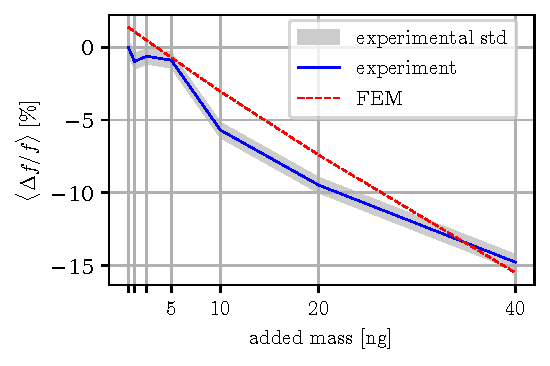
\includegraphics[]{figures/rel_freq_shift_sampled.pdf}
    \caption{Relative shifts in eigenfrequencies with increasing PS mass averaged over all modes excluding $(3,1)$. Simulation results compared with experimental data.}
    \label{fig:relative_shift_eigenfrequency}
\end{figure}
















The objective of this thesis is to establish a numerical model which allows the sample mass to be inferred from a measured resonance frequency. In other words, we seek a mass-estimation map
\begin{equation*}
    \hat m = \hat m(f_{s,\mathrm{FEM}}),
\end{equation*}
where \(f_{s,\mathrm{FEM}}\) denotes the simulated resonance frequency of the sampled membrane as defined above.

For a given membrane, let \(f_u\) denote the resonance frequency of the unsampled membrane and let \(f_{s,\mathrm{exp}}\) denote the experimentally measured resonance frequency after sample deposition. The FEM model is evaluated for different sample masses until the simulated sampled frequency matches the measured one,
\begin{equation*}
    f_{s,\mathrm{FEM}}(m_{\mathrm{FEM}}) = f_{s,\mathrm{exp}} .
\end{equation*}
The corresponding mass \(m_{\mathrm{FEM}}\) is then used as the model prediction for the sample mass.

The expected accuracy of this procedure for polystyrene samples can be estimated from Fig.~\ref{fig:relative_shift_eigenfrequency}. There, the experimentally measured and numerically simulated relative frequency shifts are represented by the functions
\begin{equation*}
    f_{r,\mathrm{exp}}(m)
    \qquad \text{and} \qquad
    f_{r,\mathrm{FEM}}(m_\mathrm{FEM}),
\end{equation*}
respectively. The inverse of the FEM relation defines the mass-estimation function,
\begin{equation*}
    \hat m(f_r) = f_{r,\mathrm{FEM}}^{-1}(f_r).
\end{equation*}
The uncertainty of this inverse map can be obtained from the uncertainty in \(f_{r,\mathrm{FEM}}\) by Gaussian error propagation. Using the inverse function theorem,
\begin{equation*}
    \frac{\mathrm d \hat m}{\mathrm d f_r}
    =
    \frac{1}{\left. \dfrac{\mathrm d f_{r,\mathrm{FEM}}}{\mathrm d m} \right|_{m=\hat m(f_r)}} ,
\end{equation*}
an uncertainty \(\Delta f_r\) in the relative frequency shift leads to a mass uncertainty
\begin{equation*}
    \Delta m
    =
    \left|
    \frac{\mathrm d \hat m}{\mathrm d f_r}
    \right|
    \Delta f_r
    =
    \frac{\Delta f_r}
    {\left| \dfrac{\mathrm d f_{r,\mathrm{FEM}}}{\mathrm d m} \right|} .
\end{equation*}
In practice, the derivative \(\mathrm d f_{r,\mathrm{FEM}}/\mathrm d m\) is approximated by finite differences.

As shown in Fig.~\ref{fig:relative_shift_eigenfrequency}, the slope of \(f_{r,\mathrm{FEM}}(m)\) is approximately constant in the considered mass range. The finite-difference estimate gives
\begin{equation*}
    \frac{\mathrm d f_{r,\mathrm{FEM}}}{\mathrm d m}
    \approx
    \SI{0.4}{\percent\per\nano\gram}.
\end{equation*}
In the ideal case, the FEM results would agree with the experimental data within the experimental standard deviation. The uncertainty in the relative frequency shift would then be approximately
\begin{equation*}
    \Delta f_r \approx \SI{0.5}{\percent},
\end{equation*}
which yields an ideal mass resolution of
\begin{equation*}
    \Delta m_{\mathrm{ideal}}
    \approx
    \frac{\SI{0.5}{\percent}}
         {\SI{0.4}{\percent\per\nano\gram}}
    =
    \SI{1.25}{\nano\gram}.
\end{equation*}
For the present, non-ideal agreement between simulation and experiment, the relevant frequency-shift error is estimated by
\begin{equation*}
    \Delta f_r
    =
    \left|
    f_{r,\mathrm{FEM}} - f_{r,\mathrm{exp}}
    \right| .
\end{equation*}
In the worst case considered here, this deviation is approximately \(\SI{2}{\percent}\). This corresponds to a realistic current mass uncertainty of
\begin{equation*}
    \Delta m_{\mathrm{current}}
    \approx
    \frac{\SI{2}{\percent}}
         {\SI{0.4}{\percent\per\nano\gram}}
    =
    \SI{5}{\nano\gram}.
\end{equation*}

Consequently, the best achievable accuracy under the present experimental conditions is estimated to be approximately
\begin{equation*}
    \Delta m_{\mathrm{ideal}} \approx \pm \SI{1.25}{\nano\gram}.
\end{equation*}
Due to the remaining discrepancy between the FEM model and the measurements, the current practical accuracy is instead approximately
\begin{equation*}
    \Delta m_{\mathrm{current}} \approx \pm \SI{5}{\nano\gram}.
\end{equation*}
This accuracy could be improved substantially by a more detailed investigation of the influence of the sample position. However, for the present experimental uncertainty, the achievable mass accuracy remains bounded from below by approximately \(\pm \SI{1.25}{\nano\gram}\). The above accuracy estimates apply specifically to the polystyrene samples considered here. As discussed in the following section, additional complications arise for other sample materials.











\subsection{Polypropylene}
\label{sec:polypropylene}

The results in this section were generated with \texttt{sample\_prestress\_analysis.ipynb}. As shown in Figure \ref{fig:mass_response} (B), the resonance frequencies of membranes with PP deposits exhibit almost no systematic shifts, regardless of the sample mass. This stands in contrast to the PS case. We model this behavior by introducing prestress in the deposited PP material. With this modification, the simulations reproduce the experimental trends more accurately. Nevertheless, this outcome highlights a fundamental limitation: if the deposition does not induce measurable frequency shifts, then the eigenfrequency response cannot provide predictive information about the deposited mass.\\


\begin{figure}[h]
    \centering
    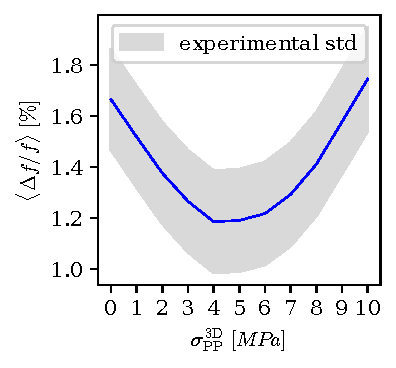
\includegraphics[]{figures/sample_prestress_analysis.pdf}
    \caption{Average deviation between simulated and measured eigenfrequencies of PP-sampled membranes as a function of assumed sample prestress $\sigma_{PP}^{3D}$. While the agreement improves around \SI{5}{\mega\pascal}, the values remain within relatively large error margins.}
    \label{fig:prestress_analysis}
\end{figure}


We first simulated the PP deposits with default parameters and zero prestress, as for PS. In this case (Figure \ref{fig:PP_eigenfreqs}A), the eigenfrequencies decrease with increasing mass, in clear disagreement with experiment. Microscopy showed that the coffee ring for the \SI{10}{\nano\gram} sample had a smaller radius ($\SI{170}{\micro\meter}$) compared to the other samples ($\SI{250}{\micro\meter}$). Incorporating this reduced radius into the simulation already accounts for part of the stagnation in eigenfrequencies (Figure \ref{fig:PP_eigenfreqs}B). After this, the second modes fit the experimental data better, but the third modes fit worse. Further agreement was achieved by introducing a sample prestress, with an optimal fit at $\sigma_{PP}^{3D}=\SI{5}{\mega\pascal}$ (Figure \ref{fig:PP_eigenfreqs}C). The corresponding analysis of the deviation as a function of prestress is shown in Figure \ref{fig:prestress_analysis}.\\



Finally, we investigated whether a sufficiently large sample prestress could even lead to an \textit{increase} in eigenfrequencies upon sampling. Using the mass density of PP and the fitted $\sigma_\silnit$, we found that such a reversal occurs at approximately $\sigma_{PP}^{3D}=\SI{8}{\mega\pascal}$. To illustrate this effect, Figure \ref{fig:PP_eigenfreqs} (D) shows the extreme case of a hypothetical prestress of $\SI{50}{\mega\pascal}$, where the sampled material effectively stiffens the membrane.\\

\newpage

\begin{figure}[h]
    \begin{overpic}[]{figures/fem_freqs_sampled_prestress_fixed_0.pdf}
        \put(10,51){\large\bfseries\textcolor{black}{A}}
    \end{overpic}\\
    \begin{overpic}[]{figures/fem_freqs_sampled_prestress_variable_0.pdf}
        \put(15,76){\large\bfseries\textcolor{black}{B}}
    \end{overpic}
    \begin{overpic}[]{figures/fem_freqs_sampled_prestress_variable_5000000.0.pdf}
        \put(9,79){\large\bfseries\textcolor{black}{C}}
    \end{overpic}\\
    \begin{overpic}[]{figures/fem_freqs_sampled_prestress_fixed_50000000.0.pdf}
        \put(15,81){\large\bfseries\textcolor{black}{D}}
    \end{overpic}
    \caption{Simulated eigenfrequencies for membranes with PP deposits under varying assumptions of sample prestress $\sigma_{PP}^{3D}$. (\textbf{A}) Zero prestress, fixed sample radius $R_\mathrm{samp}=\SI{250}{\micro\meter}$. (\textbf{B}) Zero prestress with variable radius, reduced to $R_\mathrm{samp}=\SI{170}{\micro\meter}$ at \SI{10}{\nano\gram}. (\textbf{C}) Optimal fit with $\sigma_{PP}^{3D}=\SI{5}{\mega\pascal}$ and variable radius. (\textbf{D}) Hypothetical case with $\sigma_{PP}^{3D}=\SI{50}{\mega\pascal}$, illustrating how a highly prestressed deposit could stiffen the membrane. In some cases the mode detection algorithm failed to identify the $(1,3)$ mode (notably at \SI{5}{} and \SI{10}{\nano\gram}).}
    \label{fig:PP_eigenfreqs}
\end{figure}

\clearpage


\section{Conclusions and outlook}

The aim of this thesis was to assess whether a mechanical FEM simulation of the EMILIE device can accurately predict the deposited mass from its eigenfrequency response. We find that, within the limitations of the present model, this is only feasible for relatively large sample masses (\SI{10}{\nano\gram} and above) and not for all materials. However, a simulation framework for improved estimation of the membrane prestress could be established.\\
In principle, it should also be possible to infer the spatial distribution of the deposited mass from a given set of eigenfrequencies. This could be achieved by constructing a database of simulated frequency responses for a wide range of mass distributions. Experimental data could then be matched to the database to identify the most likely distribution. For sample masses above \SI{10}{\nano\gram}, the present results suggest that this approach is viable. Importantly, generating such a database would be straightforward with the framework developed in this thesis and would not require excessive computational resources.\\

\newpage